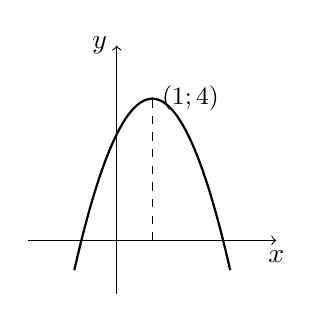
\begin{tikzpicture}[scale=0.45]
    \draw[->] (-2.5,0) -- (4.5,0) node[below] {$x$};
    \draw[->] (0,-1.5) -- (0,5.5) node[left] {$y$};

    \draw[dashed] (1,0) -- (1,4);
    \draw[thick, domain=-1.2:3.2, samples=200] plot (\x,{-((\x-1)^2)+4});

    \fill (1,4) circle (1.2pt);
    \node[right] at (1,4) {\small $(1;4)$};
\end{tikzpicture}
